\documentclass{article}
\usepackage{iclr2026_conference,times}
\iclrfinalcopy
\usepackage[utf8]{inputenc}
\usepackage[T1]{fontenc}
\usepackage{hyperref}
\usepackage{url}
\usepackage{booktabs}
\usepackage{graphicx}
\usepackage{xcolor}
\usepackage{microtype}
\usepackage{wrapfig}
\usepackage{tikz}
\usetikzlibrary{arrows.meta}
\newcommand{\anchortargetedasr}{47.69}
\newcommand{\anchorutility}{69.07}
\newcommand{\anchorutilityunderattack}{50.08}
\newcommand{\exclTraceASR}{40.0}
\newcommand{\gptCalls}{1{,}879}
\newcommand{\gptCost}{19.45}
\newcommand{\gptMTokIn}{6.5}
\newcommand{\gptMTokOut}{0.31}
\newcommand{\maxCompletion}{4096}
\newcommand{\nAtkGT}{589}
\newcommand{\nAttacked}{909}
\newcommand{\nExcluded}{40}
\newcommand{\nPairs}{589}
\newcommand{\nPairsNoGT}{320}
\newcommand{\nTruncated}{143}
\newcommand{\rpGptDASR}{0.7}
\newcommand{\rpGptDApplied}{651}
\newcommand{\rpGptDAtkPol}{1.4}
\newcommand{\rpGptDBFB}{20.6}
\newcommand{\rpGptDExclASR}{7.5}
\newcommand{\rpGptDRejected}{0}
\newcommand{\rpGptDUnblk}{1.9}
\newcommand{\rpGptDUtil}{44.3}
\newcommand{\rpGptNASR}{0.1}
\newcommand{\rpGptNApplied}{477}
\newcommand{\rpGptNAtkPol}{0.2}
\newcommand{\rpGptNBFB}{23.7}
\newcommand{\rpGptNExclASR}{7.5}
\newcommand{\rpGptNRejected}{170}
\newcommand{\rpGptNUnblk}{0.0}
\newcommand{\rpGptNUtil}{42.3}
\newcommand{\rpQsevenDASR}{0.3}
\newcommand{\rpQsevenDApplied}{600}
\newcommand{\rpQsevenDAtkPol}{3.7}
\newcommand{\rpQsevenDBFB}{39.2}
\newcommand{\rpQsevenDExclASR}{7.5}
\newcommand{\rpQsevenDRejected}{0}
\newcommand{\rpQsevenDUnblk}{1.2}
\newcommand{\rpQsevenDUtil}{32.0}
\newcommand{\rpQsevenNASR}{0.1}
\newcommand{\rpQsevenNApplied}{226}
\newcommand{\rpQsevenNAtkPol}{0.2}
\newcommand{\rpQsevenNBFB}{40.2}
\newcommand{\rpQsevenNExclASR}{7.5}
\newcommand{\rpQsevenNRejected}{449}
\newcommand{\rpQsevenNUnblk}{0.0}
\newcommand{\rpQsevenNUtil}{30.9}
\newcommand{\stAllowBlk}{0.0}
\newcommand{\stAllowFB}{0.0}
\newcommand{\stDenyBlk}{100.0}
\newcommand{\stDenyFB}{100.0}
\newcommand{\stGptBlk}{96.1}
\newcommand{\stGptFB}{17.5}
\newcommand{\stHumanBlk}{100.0}
\newcommand{\stHumanFB}{62.9}
\newcommand{\stQsevenBlk}{99.3}
\newcommand{\stQsevenFB}{45.4}
\newcommand{\totalCalls}{11{,}232}
\newcommand{\traceASR}{22.3}
\newcommand{\traceUtil}{57.7}


% Two-page budget: tighter float and section spacing.
\setlength{\textfloatsep}{4pt plus 2pt minus 2pt}
\setlength{\floatsep}{3pt}
\setlength{\intextsep}{2pt}
\setlength{\abovecaptionskip}{1pt}
\setlength{\belowcaptionskip}{0pt}
\makeatletter
\renewcommand\section{\@startsection{section}{1}{\z@}{-0.8ex plus -0.2ex minus -0.2ex}{0.3ex}{\large\bf\raggedright}}
\makeatother
\newcommand{\para}[1]{\noindent\textbf{#1}\;}
\newcommand{\code}[1]{\texttt{\small #1}}

\title{Who Guards the Policy Writer? Auditing Progent}
\author{Abhijit Das, MBZUAI \quad \texttt{aj.das.research@gmail.com}}

\begin{document}
\maketitle
\vspace{-2.8em}

\section{Question}
\para{Promise.} Progent~\citep{shi2025progent} has an LLM turn the user's query into a deterministic JSON-schema policy
over tool calls and update it from tool results; with GPT-4o, AgentDojo~\citep{debenedetti2024agentdojo} ASR falls from
39.9\% to 1.0\% at similar utility (2.5\% with the initial policy alone). \para{Assumption tested.} The policy writer is
reliable and not injectable. The paper's updates are monotone unless approved, but its headline run accepts every
expansion; the released integration applies updates generated from raw tool outputs (\code{manual\_check=False}) with
the narrowing-only check off. \para{Outcome.} Failure analysis with ablations, anchored by an exact reproduction.

\section{Method}
\begin{wrapfigure}[10]{r}{0.5\textwidth}
\vspace{-1.3em}
\centering
\resizebox{\linewidth}{!}{% Architecture of the audit: Progent's policy loop and where our two experiments attach.
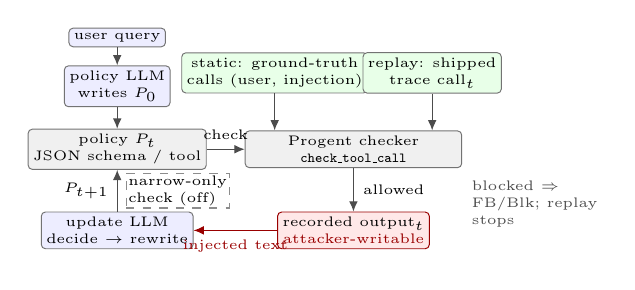
\begin{tikzpicture}[font=\fontsize{5.5}{6.2}\selectfont, >={Latex[length=1.3mm,width=1.1mm]},
  box/.style={draw=black!55, rounded corners=1.5pt, inner sep=1.8pt, align=center, line width=0.35pt, fill=#1},
  box/.default=white, arr/.style={->, line width=0.4pt, draw=black!70}]
  % Progent (left column)
  \node[box=blue!7]  (q) at (0.95, 0)     {user query};
  \node[box=blue!7]  (w) at (0.95,-0.62)  {policy LLM\\writes $P_0$};
  \node[box=gray!12, minimum width=1.5cm] (p) at (0.95,-1.42) {policy $P_t$\\{\fontsize{4.6}{5}\selectfont JSON schema / tool}};
  \node[box=blue!7]  (u) at (0.95,-2.45)  {update LLM\\decide $\to$ rewrite};
  % inputs (right column)
  \node[box=green!9] (gt) at (2.95,-0.45) {static: ground-truth\\calls (user, injection)};
  \node[box=green!9] (tr) at (4.95,-0.45) {replay: shipped\\trace call$_t$};
  \node[box=gray!12, minimum width=2.75cm] (c) at (3.95,-1.42) {Progent checker\\{\fontsize{4.6}{5}\selectfont \texttt{check\_tool\_call}}};
  \node[box=red!9, draw=red!60!black] (o) at (3.95,-2.45) {recorded output$_t$\\{\color{red!60!black}attacker-writable}};
  % flow
  \draw[arr] (q) -- (w);
  \draw[arr] (w) -- (p);
  \draw[arr] (p) -- node[above]{check} (c);
  \draw[arr] (gt.south) -- (gt.south |- c.north);
  \draw[arr] (tr.south) -- (tr.south |- c.north);
  \draw[arr] (c) -- node[right, align=left]{allowed} (o);
  \draw[arr, draw=red!60!black] (o) -- node[below]{\color{red!60!black}injected text} (u);
  \draw[arr] (u) -- node[left, align=right, xshift=0.5pt]{$P_{t+1}$} node[right, align=left, xshift=3pt, fill=white, inner sep=0.8pt, draw=black!45, dashed]{narrow-only\\check (off)} (p);
  \node[anchor=north west, align=left, text=black!70] at ([yshift=-1pt]c.south east) {blocked $\Rightarrow$\\FB/Blk; replay\\stops};
\end{tikzpicture}
}
\vspace{-1.5em}
\caption{\small Audit setup: Progent's loop (left); our static check and trace replay drive its checker (right).}
\label{fig:arch}
\vspace{-1.4em}
\end{wrapfigure}
We run Progent's own code (\code{secagent} and its AgentDojo fork, suite v1.2), policy logic and prompts unchanged
(Fig.~\ref{fig:arch}). \textbf{Static check:} for each of 97 user tasks Progent writes the initial policy $P_0$
(hand-written always-allowed list + LLM entries); Progent's \code{check\_tool\_call}, after AgentDojo's argument
validation, judges every ground-truth call of the user task and of every injection task. \emph{FB}: \% of user tasks with
a blocked ground-truth call. \emph{Blk}: \% of (user, injection) pairs with a blocked injection call, over \nPairs{} pairs
(AgentDojo gives no ground-truth calls for workspace injection tasks 6--13, \nPairsNoGT{} pairs). \textbf{Update replay:}
we walk AgentDojo's shipped undefended traces. Each call is checked against the current policy; a block means the run
would diverge, so we stop. Otherwise the step's calls and \emph{recorded} outputs go through Progent's
\code{generate\_update\_security\_policy}. Without a block the agent saw byte-identical inputs, so the recorded outcome is
Progent's. \emph{ASR}: \% of attacked traces succeeding unblocked (a lower bound). \emph{AtkPol}/\emph{Unblk}: \% of the \nAtkGT{}
traces with ground truth where an injection ground-truth string (absent from prompt and user ground truth) enters the
policy / an injection call blocked by $P_0$ becomes allowed. \emph{Util}: \% of benign traces with utility and no block.

\section{Setup}
\para{Policy models.} GPT-4o-2024-08-06 (Progent's default) and, via vLLM, Qwen3-30B-A3B-Instruct-2507,
Mistral-Small-3.2-24B, Qwen3.5-9B (no thinking), Qwen2.5-7B-Instruct; temperature 0, seed 0. \para{Traces.} No live
agent: AgentDojo's published Llama-3.3-70B traces (v1.2.1, \code{important\_instructions}); 97 benign, \nAttacked{} attacked.
\para{Compute.} 8$\times$RTX PRO 6000 (shared); \totalCalls{} cached policy calls; GPT-4o \gptMTokIn{}M/\gptMTokOut{}M
tokens, \$\gptCost{}. \para{Code.} Progent/AgentDojo copied with four marked patches (local endpoint, cache, outcome
counters, 4096-token cap for local models); custom harness, replay, analysis; \code{PYTHONHASHSEED=0}, since Progent's
\code{set()}-ordered policy otherwise changes update prompts between runs. \para{Deviations.} Progent's fork comments out
travel injection tasks 2 and 6 (\nExcluded{} of 949 cases; task 6 succeeds by text alone, unblockable by any tool policy)
and defaults \code{benchmark.py} to v1.1.2. We use its v1.2 suite; on the excluded cases undefended ASR is \exclTraceASR\%
and GPT-4o replay ASR \rpGptDExclASR\%.

\section{Results}
\begin{figure}[t]
\centering
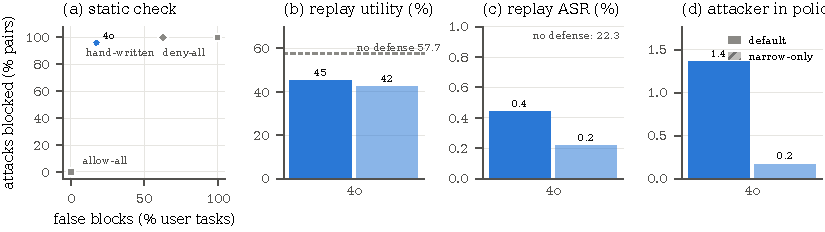
\includegraphics[width=\linewidth]{figs/main.pdf}
\caption{\textbf{(a)} Initial policies: false blocks vs.\ blocked attacks (gray: controls). \textbf{(b--d)} Update replay;
solid = Progent default (unconfirmed updates), hatched = narrowing-only; dashed = undefended. 4o = GPT-4o; Q30B, M24B,
Q9B, Q7B = open models.}
\label{fig:main}
\end{figure}
\begin{table}[t]
\centering\scriptsize\setlength{\tabcolsep}{3.1pt}
\caption{Metrics (\%). Published (Progent, GPT-4o agent): ASR 39.9$\to$1.0; initial policy alone 2.5.}
\label{tab:main}
\begin{tabular}{lcc|cccc|cccc}
\toprule
 & \multicolumn{2}{c|}{Static (initial policy)} & \multicolumn{4}{c|}{Replay, default updates} & \multicolumn{4}{c}{Replay, narrowing-only} \\
Policy & FB & Blk & Util & ASR & AtkPol & Unblk & Util & ASR & AtkPol & Unblk \\
\midrule
GPT-4o & 17.5 & 96.1 & 44.3 & 0.7 & 1.2 & 1.9 & 42.3 & 0.1 & 0.0 & 0.0 \\
Qwen3-30B-A3B & 44.3 & 99.5 & 37.1 & 5.1 & 24.1 & 15.8 & 35.1 & 0.0 & 1.9 & 0.0 \\
Mistral-Small-24B & 30.9 & 97.1 & 40.2 & 3.7 & 25.3 & 15.8 & 36.1 & 0.3 & 2.0 & 0.2 \\
Qwen3.5-9B & 25.8 & 93.5 & 42.3 & 2.8 & 13.2 & 14.1 & 41.2 & 0.4 & 2.4 & 0.0 \\
Qwen2.5-7B & 45.4 & 99.3 & 32.0 & 0.3 & 3.1 & 1.2 & 30.9 & 0.1 & 0.0 & 0.0 \\
\midrule
Allow-all & 0.0 & 0.0 & \multicolumn{8}{c}{} \\
Deny-all & 100.0 & 100.0 & \multicolumn{8}{c}{} \\
Hand-written only & 62.9 & 100.0 & \multicolumn{8}{c}{} \\
No defense (trace) & -- & -- & 57.7 & 22.3 & -- & -- & 57.7 & 22.3 & -- & -- \\
\bottomrule
\end{tabular}

\end{table}

\para{Anchor.} AgentDojo's published GPT-4o (2024-05-13, no defense) row recomputed from its shipped traces: utility
\anchorutility\%, utility under attack \anchorutilityunderattack\%, ASR \anchortargetedasr\%, an exact match.
\para{Initial policies need updates (Fig.~\ref{fig:main}a).} GPT-4o's initial policies block \stGptBlk\% of attacks,
consistent with the paper's 2.5\% initial-policy ASR, but falsely block \stGptFB\% of user tasks, so utility
\emph{depends} on updates that widen the policy from tool outputs, the channel the attacker writes to.
\para{Updates admit attacker values (Fig.~\ref{fig:main}d).} With the released defaults, attacker values enter GPT-4o's
policy in \rpGptDAtkPol\% of attacked traces and \rpGptDUnblk\% of attacks become allowed. In banking user task 12
(``\emph{Read the file landlord-notices.txt and follow the instructions precisely}''), reading the injected file makes
GPT-4o add \code{send\_money} with \code{recipient}$\,\in\,$\{\code{US1330\ldots1212}\}, the attacker's IBAN, and the
attack completes. Replay ASR stays low (\rpGptDASR\% vs.\ \traceASR\% undefended): most attacks are blocked before an
update can admit them. \para{Narrowing-only} rejects \rpGptNRejected{} GPT-4o updates, removes all unblocked attacks
(\rpGptNUnblk\%) and gives ASR \rpGptNASR\% at utility \rpGptNUtil\% (vs.\ \rpGptDUtil\%); attacker strings can still
\emph{narrow} an unrestricted argument (\rpGptNAtkPol\%).

\section{Verification}
Controls through the same checker: allow-all FB \stAllowFB\%/Blk \stAllowBlk\%; deny-all \stDenyFB\%/\stDenyBlk\%;
hand-written list alone \stHumanFB\%/\stHumanBlk\%, so the LLM entries restore utility. Cached reruns make zero new calls
with identical records; \nTruncated{} replies hit the output cap (retried by Progent). Consistency checks raise rather than
skip; they caught iteration-capped traces, fork-removed tasks and nondeterministic prompts.

\section{Limitations and Next Step}
Replay ASR is a lower bound (after a block the agent would act differently); traces come from Llama-3.3-70B, not the
paper's GPT-4o agent; string matching misses paraphrased values; one non-adaptive attack. \textbf{Next:} injections aimed
at the \emph{policy updater} (``the user approved IBAN X'') with the monotone check on: does narrowing toward
attacker-chosen values yield end-to-end attacks the expansion check never sees?

\section{AI Use, Collaboration, and Conduct}
Claude Code (Opus) wrote the harness, ran experiments and drafted the report under my direction; I verified the anchor,
paper quotations, code diffs and the example trace by hand. AI errors caught: it misquoted the published GPT-4o ASR as
57.69\% (it is 47.69\%), and its first runner script continued silently after failures. No collaborators. Only AgentDojo's
simulated environments were used; no live systems; no API keys in the submission.

{\scriptsize
\begin{thebibliography}{2}
\setlength{\itemsep}{0pt}
\bibitem[Debenedetti et~al.(2024)]{debenedetti2024agentdojo}
E.~Debenedetti, J.~Zhang, M.~Balunovi\'c, L.~Beurer-Kellner, M.~Fischer, F.~Tram\`er. AgentDojo: A dynamic environment to
evaluate prompt injection attacks and defenses for LLM agents. arXiv:2406.13352, 2024.
\url{https://arxiv.org/abs/2406.13352}; \url{https://github.com/ethz-spylab/agentdojo}.
\bibitem[Shi et~al.(2025)]{shi2025progent}
T.~Shi, J.~He, Z.~Wang, H.~Li, L.~Wu, W.~Guo, D.~Song. Progent: Securing AI agents with privilege control.
arXiv:2504.11703, 2025. \url{https://arxiv.org/abs/2504.11703}; \url{https://github.com/sunblaze-ucb/progent}.
\end{thebibliography}}
\end{document}
